% =============================================================================
% Results & Evaluation — single self-contained LaTeX file
% Compile: pdflatex results_evaluation.tex   (from paper/ directory)
% Embed in IEEEtran: copy \section{Results and Evaluation} ... \subsection{Discussion}
%   into your main paper, keep \usepackage{pgfplots}, \usepackage{booktabs}
% =============================================================================
\documentclass[10pt]{article}
\usepackage[margin=0.9in]{geometry}
\usepackage{booktabs}
\usepackage{graphicx}
\usepackage{pgfplots}
\pgfplotsset{compat=1.18}
\usepackage{amsmath}
\usepackage{xcolor}

\title{Results and Evaluation (draft fragment)}
\author{}
\date{}

\begin{document}
\maketitle

\section{Results and Evaluation}

This section documents the data we train on, how splits are built, and how three long-context strategies compare on the official held-out test portion. Numbers are taken from exported predictions and split statistics so they can be recomputed from the repository (CSV logs and \texttt{paper/experiment\_split\_distributions.json}).

\subsection{Dataset}
We use the SemEval-2026 Task~C training parquet (\texttt{task\_c\_training\_set\_1.parquet}): 900{,}000 labeled snippets with columns \texttt{code}, \texttt{generator}, \texttt{label}, and \texttt{language}. The task is to assign each snippet to one of four origins: Human (0), Machine (1), Hybrid (2), or Adversarial (3). We do not train on the full 900{,}000 rows; instead we optimize on a \textbf{length-stratified subset} so long code is not drowned out by short snippets (details below).

Table~\ref{tab:train_dist} contrasts label counts in the \textbf{full} release with those in the stratified training subset (201{,}826 rows, 22.4\% of the file; sampling in Section~\ref{sec:split_stats}). Compared with the raw corpus, the subset raises the Machine share and reduces Hybrid and Adversarial mass; Human stays the plurality class at roughly 55\% in both columns. That rebalancing is intentional: it aligns training mass more closely with the difficulty of rare or mixed-origin classes while still leaving most labels as Human.

\begin{table}[htbp]
  \centering
  \caption{Label distribution: full training file vs.\ stratified subset used for model training (same taxonomy).}
  \label{tab:train_dist}
  \begin{tabular}{@{}l rr rr@{}}
    \toprule
    & \multicolumn{2}{c}{Full file (900{,}000)} & \multicolumn{2}{c}{Training subset (201{,}826)} \\
    \cmidrule(lr){2-3} \cmidrule(lr){4-5}
    Class & Count & Share (\%) & Count & Share (\%) \\
    \midrule
    Human (0)        & 485{,}483 & 54.0 & 110{,}492 & 54.8 \\
    Machine (1)      & 210{,}471 & 23.4 &  56{,}781 & 28.1 \\
    Hybrid (2)       &  85{,}520 &  9.5 &  11{,}543 &  5.7 \\
    Adversarial (3)  & 118{,}526 & 13.2 &  23{,}010 & 11.4 \\
    \midrule
    \textbf{Total}   & 900{,}000 & 100.0 & 201{,}826 & 100.0 \\
    \bottomrule
  \end{tabular}
\end{table}

The most frequent languages in the training file are Python (249{,}247), Java (239{,}751), C\# (107{,}949), C++ (75{,}738), JavaScript (73{,}745), and Go (57{,}844), with the remainder spread across C, PHP, and others. Models therefore see a multi-language mix dominated by a few ecosystems; we do not stratify by language in the experiments reported here.

\subsection{Data splits used for training and evaluation}
\label{sec:split_stats}
All length statistics use UniXcoder tokenizer length \texttt{tok\_len}, i.e., the same tokenization the encoder sees. The training subset (target 200{,}000, seed 42) draws 20\% of rows from $\texttt{tok\_len}\leq 512$ and 80\% from longer code, with additional allocation across long-length buckets (methodology). The realized size is 201{,}826 rows because integer bucket targets need not sum to exactly 200{,}000.

Validation and test are disjoint halves of the official Task~C \emph{validation} release (33{,}743 / 33{,}742 snippets), stratified by the same short/long recipe as training. They are not random subsamples of the 900{,}k training parquet, so test performance reflects generalization to that release rather than to i.i.d.\ rows from the training file.

Table~\ref{tab:split_sizes} lists sizes and short vs.\ long counts. Table~\ref{tab:split_labels} shows that validation and test are label-shifted relative to the training subset: Human is a smaller share ($\sim$44\%) while Hybrid and Adversarial are larger ($\sim$9.7\% / $\sim$14.4\%). That makes the held-out split a stricter check than matching the training label mix. Table~\ref{tab:toklen_three} and Figure~\ref{fig:toklen_three} summarize the tokenizer-length histogram in five bins; the training subset places more mass in the 1025+ bin than validation or test (27.3\% vs.\ $\sim$18.3\%), so models are trained with a somewhat longer-tailed length distribution than the split used for headline metrics. Counts are mirrored in \texttt{paper/experiment\_split\_distributions.json}, produced by \texttt{paper/compute\_experiment\_split\_distributions.py}.

\begin{table}[htbp]
  \centering
  \footnotesize
  \setlength{\tabcolsep}{3.5pt}
  \caption{Splits (UniXcoder \texttt{tok\_len}). Tr.\,\% = training subset as a fraction of the 900{,}000-row training release; ``---'' for val/test. Short/Long = $\leq$512 / $>$512 tokens; L\% = long share of that split.}
  \label{tab:split_sizes}
  \begin{tabular}{@{}l r r r r r@{}}
    \toprule
    Split & $n$ & Tr.\,\% & $\leq$512 & $>$512 & L\% \\
    \midrule
    Training (strat.) & 201{,}826 & 22.4 & 40{,}000 & 161{,}826 & 80.2 \\
    Validation & 33{,}743 & --- & 8{,}000 & 25{,}743 & 76.3 \\
    Test & 33{,}742 & --- & 8{,}000 & 25{,}742 & 76.3 \\
    \bottomrule
  \end{tabular}
\end{table}

\begin{table}[htbp]
  \centering
  \caption{Class distribution (\%) on each split (0 Human, 1 Machine, 2 Hybrid, 3 Adversarial).}
  \label{tab:split_labels}
  \footnotesize
  \begin{tabular}{@{}lcccc@{}}
    \toprule
    Split & 0 & 1 & 2 & 3 \\
    \midrule
    Training subset & 54.75 & 28.13 & 5.72 & 11.40 \\
    Validation      & 44.44 & 31.53 & 9.69 & 14.35 \\
    Test            & 44.43 & 31.53 & 9.69 & 14.35 \\
    \bottomrule
  \end{tabular}
\end{table}

\begin{table}[htbp]
  \centering
  \caption{UniXcoder \texttt{tok\_len} histogram (\% of rows in each split).}
  \label{tab:toklen_three}
  \footnotesize
  \begin{tabular}{@{}lccc@{}}
    \toprule
    Bin (tokens) & Train subset & Validation & Test \\
    \midrule
    0--128     &  6.03 &  6.91 &  7.01 \\
    129--256   &  7.02 &  8.30 &  8.02 \\
    257--512   &  6.77 &  8.51 &  8.68 \\
    513--1024  & 52.92 & 57.93 & 57.98 \\
    1025+      & 27.27 & 18.37 & 18.31 \\
    \midrule
    Sum        & 100.00 & 100.00 & 100.00 \\
    \bottomrule
  \end{tabular}
\end{table}

\begin{figure}[htbp]
  \centering
  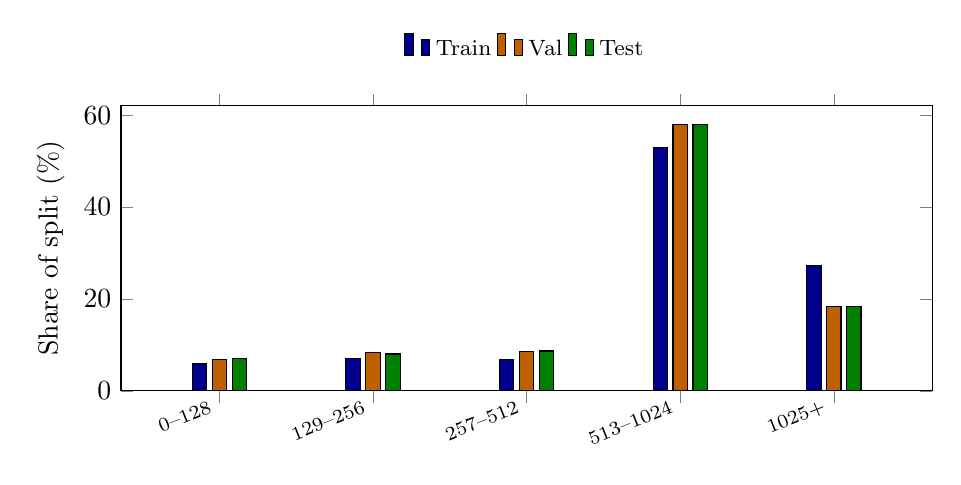
\begin{tikzpicture}
  \begin{axis}[
    width=0.98\linewidth, height=5.2cm,
    ybar,
    bar width=5.2pt,
    ymin=0, ymax=62,
    ylabel={Share of split (\%)},
    symbolic x coords={B1,B2,B3,B4,B5},
    xticklabels={0--128,129--256,257--512,513--1024,1025+},
    xtick=data,
    x tick label style={font=\scriptsize, rotate=22, anchor=east},
    enlarge x limits=0.16,
    legend style={at={(0.5,1.12)}, anchor=south, legend columns=3, draw=none, font=\footnotesize},
  ]
  \addplot[fill=blue!55!black] coordinates {(B1,6.03) (B2,7.02) (B3,6.77) (B4,52.92) (B5,27.27)};
  \addlegendentry{Train}
  \addplot[fill=orange!75!black] coordinates {(B1,6.91) (B2,8.30) (B3,8.51) (B4,57.93) (B5,18.37)};
  \addlegendentry{Val}
  \addplot[fill=green!50!black] coordinates {(B1,7.01) (B2,8.02) (B3,8.68) (B4,57.98) (B5,18.31)};
  \addlegendentry{Test}
  \end{axis}
  \end{tikzpicture}
  \caption{Tokenizer length mix for the training subset, validation, and test portions (Table~\ref{tab:toklen_three}).}
  \label{fig:toklen_three}
\end{figure}

\subsection{Experimental setup}
\label{sec:exp_setup}
We compare three ways to fit long code into a fixed encoder window. All runs share the same backbone (\texttt{microsoft/unixcoder-base}), maximum length 512, balanced class weights, the stratified training subset in Section~\ref{sec:split_stats}, and \textbf{one full training epoch} with the same optimization settings across variants (methodology). The only deliberate difference is how text is cropped or tiled before the encoder.

\textbf{Truncation} keeps the head of each snippet (single forward pass). \textbf{Multi-view} builds two crops (start and end) for long snippets, trains on both as separate labeled examples, and averages logits at evaluation time. \textbf{Sliding window} enumerates overlapping windows ($w{=}512$, $s{=}256$), trains on every window, and pools window logits back to a snippet prediction (methodology). Sliding therefore inflates the number of gradient steps per logical snippet and, at test time, typically requires more encoder calls than multi-view, which in turn uses twice as many passes as truncation on long inputs.

Headline metrics are accuracy and macro-F1 on the test partition ($n{=}33{,}742$), computed from \texttt{results/test\_inference\_*.csv} using \texttt{true\_label}, \texttt{pred\_label}, and \texttt{tok\_len} for bucketed analysis.

\subsection{Main results}
\label{sec:main_results}
Table~\ref{tab:main} reports overall accuracy and macro-averaged F1. Truncation is clearly weaker on both measures: moving from a single head crop to multi-view gains 3.43 points in accuracy (0.8621$\rightarrow$0.8964) and 4.31 points in macro-F1 (0.8167$\rightarrow$0.8598). That gap is expected when most evaluation snippets exceed 512 tokens (Table~\ref{tab:split_sizes}): the tail of the file is invisible to a single crop.

Multi-view and sliding window are \textbf{near parity} after one epoch each: sliding leads by only 0.10 percentage points in accuracy (0.8964 vs.\ 0.8974) and 0.23 points in macro-F1 (0.8598 vs.\ 0.8621). Macro-F1 is the stricter headline here because it weights the four classes equally and is sensitive to Hybrid and Adversarial errors under the label shift in Table~\ref{tab:split_labels}. The small gap between multi-view and sliding should be read together with their different training and inference costs (Section~\ref{sec:exp_setup}).

\begin{table}[htbp]
  \centering
  \caption{Held-out test set ($n{=}33{,}742$). One training epoch per model. Values from \texttt{results/test\_inference\_*.csv}.}
  \label{tab:main}
  \begin{tabular}{@{}lcc@{}}
    \toprule
    Method & Accuracy & Macro-F1 \\
    \midrule
    Truncation (single view)   & 0.8621 & 0.8167 \\
    Multi-view (start/end)     & 0.8964 & 0.8598 \\
    Sliding window ($w{=}512$, $s{=}256$) & \textbf{0.8974} & \textbf{0.8621} \\
    \bottomrule
  \end{tabular}
\end{table}

\begin{figure}[htbp]
  \centering
  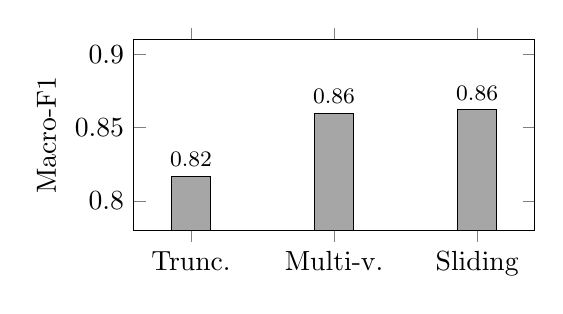
\begin{tikzpicture}
  \begin{axis}[
    width=0.55\linewidth, height=4cm,
    ybar, bar width=14pt,
    ymin=0.78, ymax=0.91,
    ylabel={Macro-F1},
    symbolic x coords={T,M,S},
    xticklabels={Trunc.,Multi-v.,Sliding},
    xtick=data,
    enlarge x limits=0.2,
    nodes near coords,
    every node near coord/.append style={font=\footnotesize},
  ]
  \addplot[fill=gray!70] coordinates {(T,0.8167) (M,0.8598) (S,0.8621)};
  \end{axis}
  \end{tikzpicture}
  \caption{Macro-F1 on the held-out test split. Multi-view and sliding differ by 0.23 points (Table~\ref{tab:main}).}
  \label{fig:macrof}
\end{figure}

\subsection{Per-class F1}
Table~\ref{tab:perclass} breaks down F1 by class. Human and Machine are the easiest labels under all three encoders, with F1 in the 0.85--0.96 range on this split. Hybrid remains the hardest row: truncation reaches only 0.7137 F1, while multi-view and sliding lift that to 0.7836 and 0.7985 respectively (roughly seven to eight and a half points absolute). Adversarial F1 improves from 0.7663 with truncation to 0.8127 / 0.8075 with multi-view / sliding, so the expensive tiling does not uniformly beat the two-crop design on every class. These patterns are consistent with Hybrid snippets occupying a narrow semantic band between Human and Machine origins.

\begin{table}[htbp]
  \centering
  \caption{Per-class F1 on the held-out test split.}
  \label{tab:perclass}
  \begin{tabular}{@{}lcccc@{}}
    \toprule
    Method & Human & Machine & Hybrid & Adv. \\
    \midrule
    Truncation   & 0.9356 & 0.8513 & 0.7137 & 0.7663 \\
    Multi-view   & 0.9610 & 0.8818 & 0.7836 & 0.8127 \\
    Sliding win. & 0.9613 & 0.8812 & 0.7985 & 0.8075 \\
    \bottomrule
  \end{tabular}
\end{table}

\subsection{Length buckets}
\label{sec:len_buckets}
To see where long-context modeling helps, we bucket test examples by \texttt{tok\_len} and recompute macro-F1 inside each bucket (Table~\ref{tab:buckets} and Figure~\ref{fig:buckets}). Performance degrades as snippets grow: all methods lose ground past $\sim$1k tokens, and the longest bucket ($\geq 2560$) is far below the short-code bins. That trend matches the intuition that labels depend on evidence spread across the file, which becomes harder to aggregate as windows multiply.

Multi-view improves macro-F1 over truncation in \emph{every} bucket, so the second crop is never harmful in this aggregate view. Sliding and multi-view are close overall: multi-view is slightly ahead in the $\leq 512$ and $[1024,1536)$ bins, while sliding leads in the dense middle bin $[512,1024)$ and on the extreme tail $\geq 2560$, where pooling many windows appears to recover a bit more signal than two fixed crops. Neither method uniformly wins across bins, which reinforces treating them as operating points on a cost--accuracy curve rather than as a strict ordering.

\begin{table}[htbp]
  \centering
  \caption{Macro-F1 by tokenizer length bucket (held-out test, same $n$ per row).}
  \label{tab:buckets}
  \footnotesize
  \begin{tabular}{@{}lccc@{}}
    \toprule
    Bucket & Trunc. & Multi-v. & Sliding \\
    \midrule
    $\leq 512$      & 0.7956 & 0.8237 & 0.8217 \\
    $[512,1024)$    & 0.7718 & 0.8421 & \textbf{0.8530} \\
    $[1024,1536)$   & 0.6716 & 0.7175 & 0.7139 \\
    $[1536,2048)$   & 0.6670 & 0.7001 & 0.6981 \\
    $[2048,2560)$   & 0.4447 & 0.4727 & 0.4809 \\
    $\geq 2560$     & 0.3166 & 0.3463 & \textbf{0.4145} \\
    \bottomrule
  \end{tabular}
\end{table}

\begin{figure}[htbp]
  \centering
  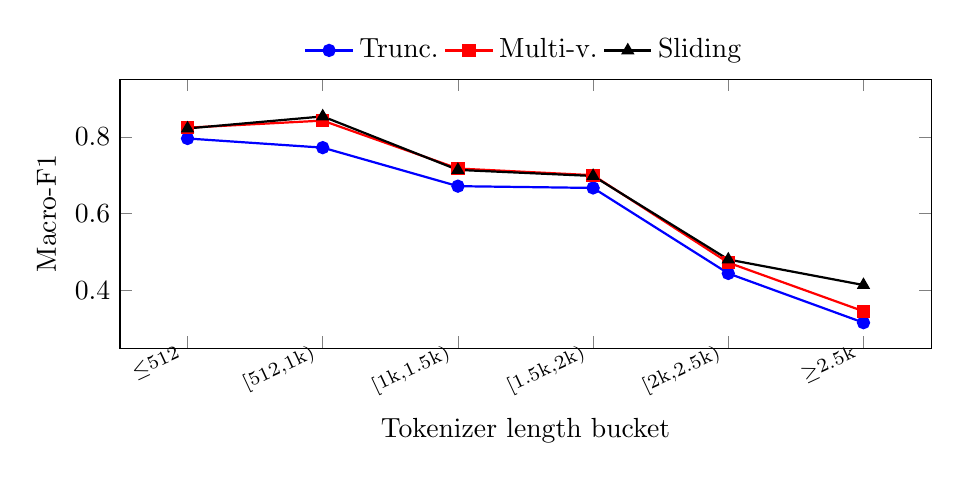
\begin{tikzpicture}
  \begin{axis}[
    width=0.98\linewidth, height=5cm,
    ylabel={Macro-F1},
    xlabel={Tokenizer length bucket},
    xmin=0.5, xmax=6.5,
    ymin=0.25, ymax=0.95,
    xtick={1,2,3,4,5,6},
    xticklabels={%
      {$\leq$512},%
      {[512,1k)},%
      {[1k,1.5k)},%
      {[1.5k,2k)},%
      {[2k,2.5k)},%
      {$\geq$2.5k}%
    },
    x tick label style={font=\scriptsize, rotate=25, anchor=east},
    legend style={at={(0.5,1.02)}, anchor=south, legend columns=3, draw=none},
  ]
  \addplot[thick, mark=*, blue] coordinates {(1,0.7956) (2,0.7718) (3,0.6716) (4,0.6670) (5,0.4447) (6,0.3166)};
  \addlegendentry{Trunc.}
  \addplot[thick, mark=square*, red] coordinates {(1,0.8237) (2,0.8421) (3,0.7175) (4,0.7001) (5,0.4727) (6,0.3463)};
  \addlegendentry{Multi-v.}
  \addplot[thick, mark=triangle*, black] coordinates {(1,0.8217) (2,0.8530) (3,0.7139) (4,0.6981) (5,0.4809) (6,0.4145)};
  \addlegendentry{Sliding}
  \end{axis}
  \end{tikzpicture}
  \caption{Macro-F1 vs.\ length bucket (Table~\ref{tab:buckets}).}
  \label{fig:buckets}
\end{figure}

\subsection{Discussion}
Taken together, the tables tell a consistent story. A single head crop leaves too much context out on an 80\%--long split, so both multi-view and sliding raise accuracy and macro-F1 sharply relative to truncation (Table~\ref{tab:main}). After \textbf{one epoch} on the stratified subset, multi-view and sliding land on nearly the same headline numbers, with sliding ahead only in the hundredths of accuracy and macro-F1. The per-class and bucket tables clarify \emph{where} the gains concentrate: Hybrid F1 is the main beneficiary of extra views (Table~\ref{tab:perclass}), and the longest snippets remain the noisiest regime for every method (Table~\ref{tab:buckets}).

The practical trade-off is computational. Sliding expands each snippet into many overlapping windows for training and inference; multi-view adds at most one extra forward pass per long snippet. Truncation stays the cheapest option and is still a useful lower bound. We trained on 22.4\% of the released 900{,}000-row parquet (Table~\ref{tab:split_sizes}); reporting on the official validation release keeps the test set independent of that file. Extending training beyond one epoch or tuning pooling could move the small gap between multi-view and sliding, but was outside the scope of the runs summarized here.

\end{document}
